% This file provides an example Beamer presentation using the RWTH theme
% showcasing some of the more common options, similar to the Powerpoint version
% 12.11.2014: Revision 1 (Harold Bruintjes, Tim Lange)

% For RWTH, beamer should be loaded with class option t (top)
\documentclass[t]{beamer}

% Use fontspec to get Arial font
% Requires use of XeLaTeX
\usepackage{fontspec}
\setmainfont{Arial}
\setsansfont{Arial}
% Also force Arial for math for a more consistent look
\usepackage{unicode-math}

% https://tex.stackexchange.com/questions/426088/texlive-pretest-2018-beamer-and-subfig-collide
\makeatletter
\let\@@magyar@captionfix\relax
\makeatother

% German style date formatting (footer)
\usepackage[ddmmyyyy]{datetime}
\renewcommand{\dateseparator}{.}

\usepackage{MnSymbol,wasysym}

% Format the captions used for figures etc.
\usepackage[compatibility=false]{caption}
\captionsetup{singlelinecheck=off,justification=raggedleft,labelformat=empty,labelsep=none}

% PGFPlots is used for drawing some of the charts
\usepackage{pgfplots}
\pgfplotsset{compat=newest}
% This file contains some styles and macros for drawing charts similar to those of MS Office

\pgfplotsset{hor_barchart/.style={
  xbar=0mm,
  xmin=0,
  xtick=\empty,
  axis y line*=left,
  x axis line style={opacity=0},
  bar width=0.6cm,
  ytick=data,
  nodes near coords,
  every axis/.append style={font=\normalsize},
  every node near coord/.append style={font=\normalsize},
  nodes near coords align={horizontal},
  legend style={at={(0,-10mm)},anchor=north west,legend columns=-1,draw=none},
}}

\pgfplotsset{ver_barchart/.style={
  ybar=0mm,
  x = 4.5cm,
  ymin=0,
  ymajorgrids,
  axis x line*=bottom,
  y axis line style={opacity=0},
  bar width=0.8cm,
  enlarge x limits={0.15},
  xtick=data,
  nodes near coords,
  every axis/.append style={font=\normalsize},
  every node near coord/.append style={font=\normalsize},
  nodes near coords align={vertical},
  legend style={at={(0,-10mm)},anchor=north west,legend columns=-1,draw=none},
}}

\tikzstyle{chart}=[
    legend label/.style={font={\normalsize},anchor=west,align=left},
    legend box/.style={rectangle, draw=none, minimum size=5pt},
]

\tikzstyle{pie chart}=[
    chart,
    slice/.style={line cap=round, line join=round,draw=none},
    pie title/.style={font={\bf}},
    slice type/.style 2 args={
        ##1/.style={fill=##2},
        values of ##1/.style={}
    }
]

\newcommand{\pie}[3][]{
    \begin{scope}[#1]
    \pgfmathsetmacro{\curA}{90}
    \pgfmathsetmacro{\r}{1}
    \def\c{(0,0)}
    \node[pie title] at (90:1.3) {#2};
    \foreach \v/\s in{#3}{
        \pgfmathsetmacro{\deltaA}{\v/100*360}
        \pgfmathsetmacro{\nextA}{\curA + \deltaA}
        \pgfmathsetmacro{\midA}{(\curA+\nextA)/2}

        \path[slice,\s] \c
            -- +(\curA:\r)
            arc (\curA:\nextA:\r)
            -- cycle;

        %\begin{pgfonlayer}{foreground}
        % Position labels at 1.2 times radius (just outside of chart)
        \path \c -- node[pos=1.2,pie values,values of \s]{$\v\%$} +(\midA:\r);
        %\end{pgfonlayer}

        \global\let\curA\nextA
    }
    \end{scope}
}

% Custom legend (used for pie chart)
\newcommand{\legend}[2][]{
\begin{scope}[#1]
  \path
    \foreach \n/\s in {#2} {
      ++(0,-5pt) node[\s,legend box] {} +(5pt,0) node[legend label] {\n}
    };
\end{scope}
}


% Load the actual RWTH theme. Suggested is to load the full theme,
% as it requires some specific dimensions
\usetheme{rwth}



% ---------------- My Stuff ---------------- %
% ---------- Hyperref ---------- %
\usepackage{hyperref}
\hypersetup{colorlinks,breaklinks,
            urlcolor=[rgb]{0,0.2,0.4},
            linkcolor=[rgb]{0,0.2,0.4}}
\def\UrlBreaks{\do\/\do-}
% Farbe ist darkmidnightblue
% ---------- -------- ---------- %

\begin{document}

\logo{
\includegraphics{logo.png}}

% Setup presentation information
\title{Back-Propagation and Algorithms for Training Artificial Neural Networks with TensorFlow}
\date{26.-30. October 2020}
\author{Gero Kauerauf}

\frame{\titlepage}

\section{List of Contents}
\begin{frame}
    \begin{itemize}
        \item Introduction
    \end{itemize}
\end{frame}


\section{Introduction}
\begin{frame}
    \begin{itemize}
        \item What is a complicated problem for a computer?
        \item A problems that is
        \begin{itemize}
            \item hard to describe formally
            \item intuitive solvable for humans
        \end{itemize}
        \item For example: Recognizing a flower on a picture
        \item Deep Learning
        \begin{itemize}
            \item Hierarchy of Concepts
            \item Representative Graph has Layers
        \end{itemize}
        \item Machine Learning
        \begin{itemize}
            \item Acquiring its own knowledge
            \item Extracting patterns from data
        \end{itemize}
    \end{itemize}
\end{frame}

\section{Data Representation}
\begin{frame}
    \begin{itemize}
        \item Importance of Data Representation
        \begin{itemize}
            \item Tasks can be impossible in one representation and easy in another
            
            \begin{figure}
                \centering
                \begin{minipage}{0.45\textwidth}
                    \centering
                    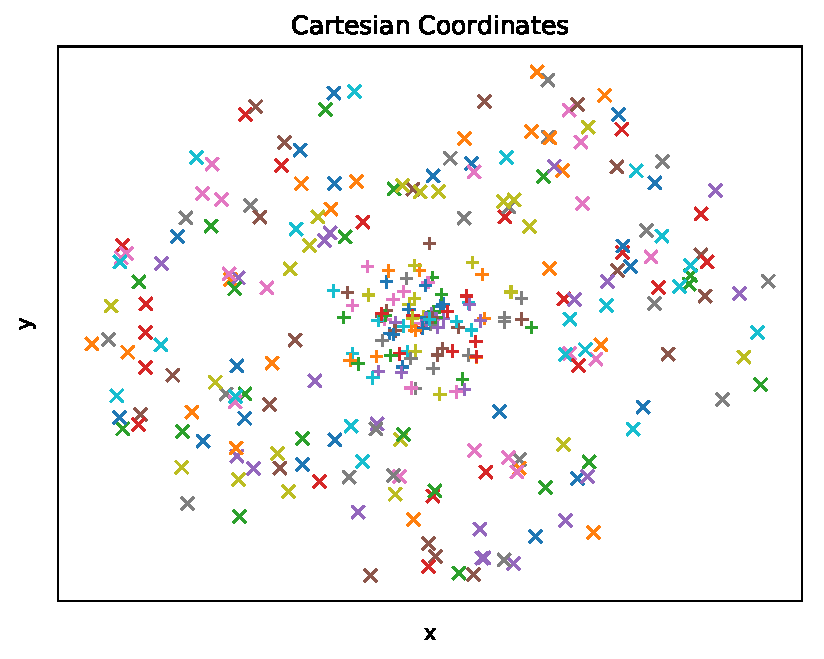
\includegraphics[width=0.9\textwidth]{../plots/cartesian.pdf} % first figure itself
                \end{minipage}\hfill
                \begin{minipage}{0.45\textwidth}
                    \centering
                    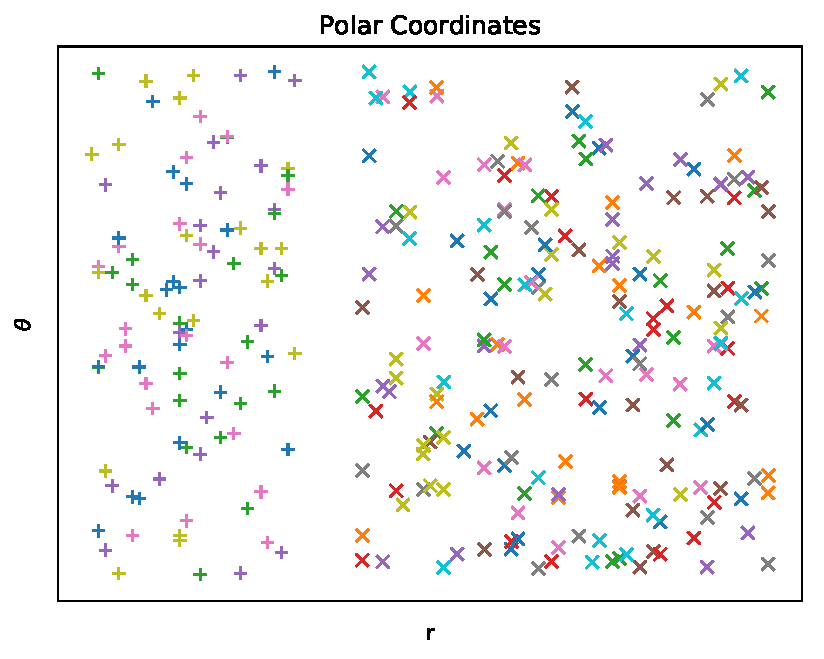
\includegraphics[width=0.9\textwidth]{../plots/polar.pdf} % second figure itself
                \end{minipage}
            \end{figure}

            \item One solution to this is \textbf{representation learning}
            \begin{itemize}
                \item Machine Learning now also discovers the representation itself
                \item Often better Performance
                \item AI can rapidly adapt to new tasks with minimal human intervention
            \end{itemize}
        \end{itemize}
    \end{itemize}
\end{frame}

\section{Different AI disciplines}
\begin{frame}
    \begin{itemize}
        \item Relations between different AI disciplines
        \begin{figure}
            %\centering
            \begin{minipage}{0.45\textwidth}
                \begin{figure}[]
                    \centering
                    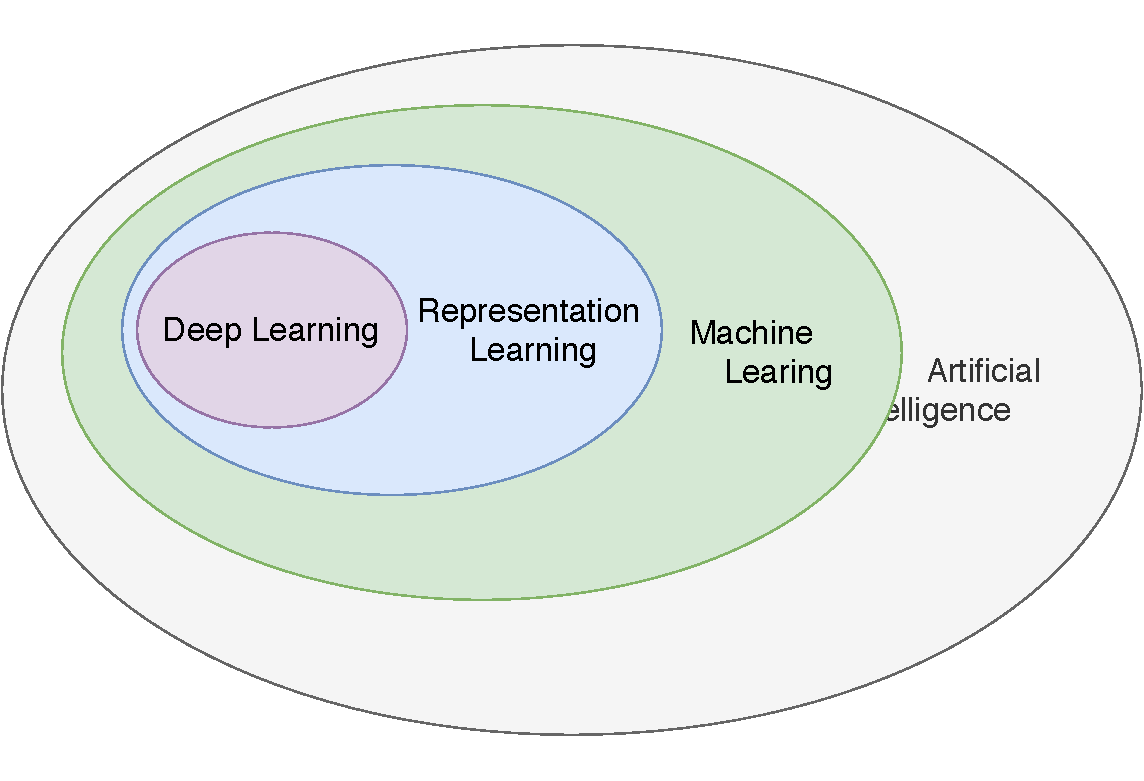
\includegraphics[width=\textwidth]{../plots/ai-venn.pdf}
                    %\caption{\href{http://www.deeplearningbook.org}{www.DeepLearningBook.org}}
                \end{figure}
            \end{minipage}\hfill
            \begin{minipage}{0.45\textwidth}
                \begin{figure}[]
                    \centering
                    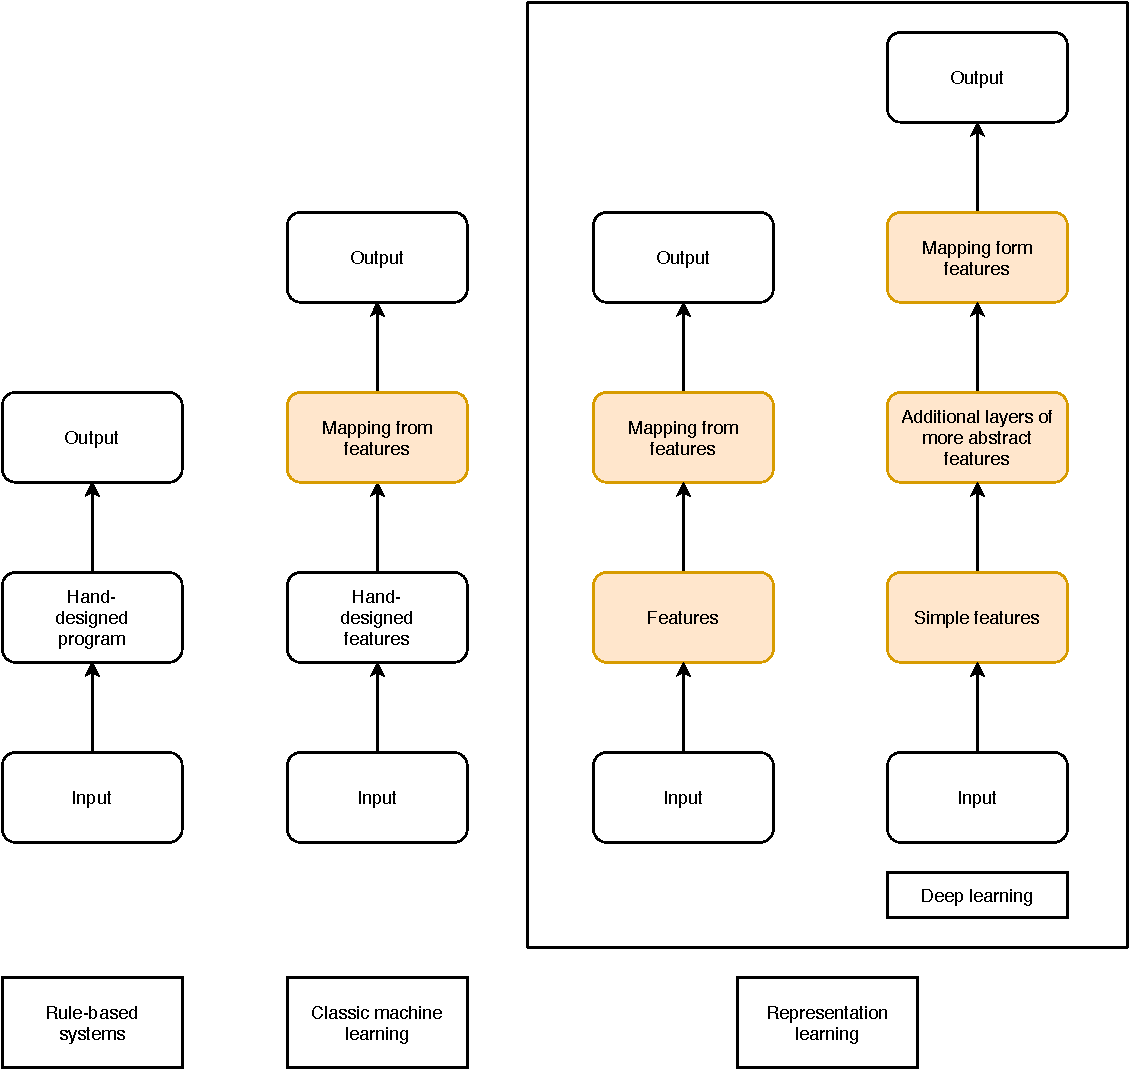
\includegraphics[width=\textwidth]{../plots/ai-flowchart.pdf}
                    %\caption{\href{http://www.deeplearningbook.org}{www.DeepLearningBook.org}}
                \end{figure}
            \end{minipage}
            \caption{\href{http://www.deeplearningbook.org}{www.DeepLearningBook.org}}
        \end{figure}
    \end{itemize}
\end{frame}

\end{document}
